\documentclass[12pt]{article} % 12pt 为字号大小 UTF8
\usepackage{amssymb,amsfonts,amsmath,amsthm}
%\usepackage{fontspec,xltxtra,xunicode}
%\usepackage{times}

%----------
% 定义中文环境
%----------

\usepackage{xeCJK}

% \setCJKmainfont[BoldFont={SimHei},ItalicFont={KaiTi}]{SimSun}
% \setCJKsansfont{SimHei}
% \setCJKfamilyfont{zhsong}{SimSun}
% \setCJKfamilyfont{zhhei}{SimHei}

% \newcommand*{\songti}{\CJKfamily{zhsong}} % 宋体
% \newcommand*{\heiti}{\CJKfamily{zhhei}}   % 黑体


%----------
% 版面设置
%----------
%首段缩进
\usepackage{indentfirst}
\setlength{\parindent}{2.1em}

%行距
\renewcommand{\baselinestretch}{1.4} % 1.4倍行距

%页边距
\usepackage[a4paper]{geometry}
\geometry{verbose,
	tmargin=3cm,% 上边距
	bmargin=3cm,% 下边距
	lmargin=3cm,% 左边距
	rmargin=3cm % 右边距
}


%----------
% 其他宏包
\usepackage{listings}

%----------
%图形相关
\usepackage[x11names]{xcolor} % must before tikz, x11names defines RoyalBlue3
\usepackage{graphicx}
\usepackage{pstricks,pst-plot,pst-eps}
\usepackage{subfig}
\def\pgfsysdriver{pgfsys-dvipdfmx.def} % put before tikz
\usepackage{tikz}

%原文照排
\usepackage{verbatim}

%网址
\usepackage{url}
\usepackage[framed,numbered,autolinebreaks,useliterate]{mcode}

%----------
% 习题与解答环境
%----------
% %习题环境
% \theoremstyle{definition} 
% \newtheorem{exs}{习题}

% %解答环境
% \ifx\proof\undefined\
% \newenvironment{proof}[1][\protect\proofname]{\par
% \normalfont\topsep6\p@\@plus6\p@\relax
% \trivlist
% \itemindent\parindent
% \item[\hskip\labelsep
% \scshape
% #1]\ignorespaces
% }{%
% \endtrivlist\@endpefalse
% }
% \fi

% \renewcommand{\proofname}{\it{证明}}

%----------
% 我的自定义
%----------

\newcommand{\horrule}[1]{\rule[0.5ex]{\linewidth}{#1}} 	% Horizontal rule

\renewcommand{\refname}{参考文献}
\renewcommand{\abstractname}{\large \bf 摘\quad 要}
\renewcommand{\contentsname}{目录}
\renewcommand{\tablename}{表}
\renewcommand{\figurename}{图}

\setlength{\parskip}{0.4ex} % 段落间距

\usepackage{enumitem}
\setenumerate[1]{itemsep=0pt,partopsep=0pt,parsep=\parskip,topsep=5pt}
\setitemize[1]{itemsep=0.4ex,partopsep=0.4ex,parsep=\parskip,topsep=0.4ex}
\setdescription{itemsep=0pt,partopsep=0pt,parsep=\parskip,topsep=5pt}


%==========
% 正文部分
%==========

\begin{document}
	\title{
		%	{\normalfont\normalsize\textsc{
		%			Xiangtan University  \\[25pt]}}
		\horrule{0.5pt}\\
		\sffamily{最优化方法上机报告\\无约束优化算法}
		\horrule{1.8pt}\\[20pt]
	}
	\author{米科润\quad 19信计二班\\201905755824}
	\date{\today} % 若不需要自动插入日期,则去掉前面的注释;{ } 中也可以自定义日期格式
	
	\begin{titlepage}
		\maketitle
		\vspace{30pt}
		\thispagestyle{empty}
	\end{titlepage}
	
	\tableofcontents
	\thispagestyle{empty}
	
	\newpage
	\setcounter{page}{1}
	
	\section{共轭梯度法}
	\subsection{线性共轭梯度法}
	输入: A是n阶对称正定矩阵,b是n维列向量,$x_0$是初始点,epsilon是容许误差,N是最大迭代次数\\
	\indent 输出: k是迭代次数,x,val分别是近似最优点和最优值
	\begin{lstlisting}
	function [k,x,val]=linecg(A,b,x0,epsilon,N)
	if nargin<5, N=1000; end
	if nargin<4, epsilon=1.e-5; end
	if nargin<3, x0=zeros(length(b),1); end
	k=0;
	gk=A*x0-b;
	dk=-gk;
	while(k<N)
		temp=A*dk;
		alpha=-gk'*dk/(dk'*temp);
		x=x0+alpha*dk;
		gk=A*x-b;
		betak=gk'*temp/(dk'*temp);
		dk=-gk+betak*dk;
		if(norm(gk)<epsilon), break; end
		x0=x;
		k=k+1;
	end
	val=0.5*x'*A*x-b'*x;
	end
	\end{lstlisting}
	\indent 结果展示:\\
	\indent 求解无约束优化问题$\underset{x\in R^n}{min} f(x)=\frac{1}{2}x^\mathrm{ T }Ax-b^\mathrm{ T }x$\\
	\indent 其中$A=\begin{pmatrix}
		4 & -1  \\
		-1 & 4 & -1 \\
		 & \ddots & \ddots & \ddots\\
		 & & -1 & 4 & -1\\
		& & & -1 & 4
		\end{pmatrix}$
	,
	$B=\begin{pmatrix}
		3 \\
		2 \\
		\vdots\\
		2\\
		3
	 \end{pmatrix}$\\
	\indent 创建运行文件test1.m
	\begin{lstlisting}
	A=zeros(100);
	A(1,1:2)=[4,-1];
	A(100,99:100)=[-1,4];
	xx=[-1,4,-1];
	for i = 2:99
		A(i,i-1:i+1)=xx;
	end
	B=2.*ones(100,1);
	B(1)=3;B(100)=3;
	x0=zeros(100,1);
	epsilon=1e-5;
	N=20;
	[k,x,val]=linecg(A,B,x0,epsilon,N);
	disp('k=');disp(k);disp('val='),disp(val);
	\end{lstlisting}
	\indent 结果如下
	\begin{figure}[ht]
		\centering
		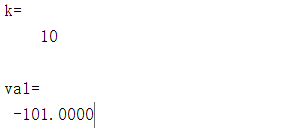
\includegraphics[width=0.45\textwidth]{xxge.png}
		\caption{线性共轭梯度法结果}
		\label{fig:fig1}
	\end{figure}
	\subsection{非线性共轭梯度法}
	\indent 基于Armijo非精确线搜索的重开始FR非线性共轭梯度法\\
	\indent 输入: fun,gfun分别是目标函数及其梯度,$x_0$是初始点,
	epsilon是容许误差,N是最大迭代次数\\
	\begin{lstlisting}
	function [k,x,val] = frcg(fun,gfun,x0,epsilon,N)
	if nargin<5, N=1000; end
	if nargin<4, epsilon=1.e-5; end
	beta=0.6; sigma=0.4;
	n=length(x0); k=0;
	while(k<N)
		gk=feval(gfun,x0); 
		itern=k-(n+1)*floor(k/(n+1));
		itern=itern+1;
		if(itern==1)
			dk=-gk;
		else
			betak=(gk'*gk)/(g0'*g0);
			dk=-gk+betak*d0; gd=gk'*dk;
			if(gd>=0.0), dk=-gk; end
		end
		if(norm(gk)<epsilon), break; end
		m=0; mk=0;
		while(m<20) 
			if(feval(fun,x0+beta^m*dk)...
					<=feval(fun,x0)+sigma*beta^m*gk'*dk)
				mk=m; break;
			end
			m=m+1;
		end
		x=x0+beta^mk*dk;
		g0=gk; d0=dk;
		x0=x;  k=k+1;
	end
	val=feval(fun,x);
	end
	\end{lstlisting}
	结果展示:\\
	\indent 求解无约束优化问题 $\underset{x\in R^2}{min} f(x)=2x_1^2+x_2^2-2x_1x_2-2x_2$\\
	\indent 编写目标函数fun1.m和梯度gfun1.m
	\begin{lstlisting}
	function f=fun1(x)
	f=2*x(1)^2+x(2)^2-2*x(1)*x(2)-2*x(2);
	end
	\end{lstlisting}
	\begin{lstlisting}
	function gf=gfun1(x)
	gf=[4*x(1)-2*x(2);2*x(2)-2*x(1)-2];
	end
	\end{lstlisting}
	\indent 命令窗口输入:
	\begin{lstlisting}
	>> x0=[0.0;0.0];
	>> [k,x,val]=frcg('fun1','gfun1',x0)
	\end{lstlisting}
	\indent 结果:
	\begin{figure}[ht]
		\centering
		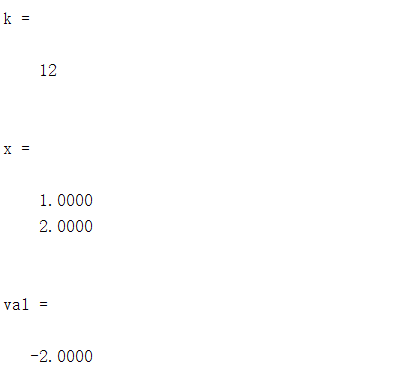
\includegraphics[width=0.45\textwidth]{fxxge.png}
		\caption{非线性共轭梯度法结果}
		\label{fig:fig1}
	\end{figure}
	\section{拟牛顿法}
	\subsection{对称秩1算法}
	\indent 输入: fun,gfun分别是目标函数及其梯度,$x_0$是初始点,
epsilon是容许误差,N是最大迭代次数\\
	\indent 输出:k是迭代次数,x,val分别是近似最优点和最优值
	\begin{lstlisting}
	function [k,x,val] = sr1(fun,gfun,x0,epsilon,N)
	if nargin<5, N=1000; end
	if nargin<4, epsilon=1.e-5; end
	beta=0.55; sigma=0.4;
	n=length(x0); Hk=eye(n); k=0;
	while(k<N)
		gk=feval(gfun,x0);
		dk=-Hk*gk;
		if(norm(gk)<epsilon), break; end 
		m=0; mk=0;
		while(m<20)
			if(feval(fun,x0+beta^m*dk)<=feval(fun,x0)...
			+sigma*beta^m*gk'*dk)
				mk=m; break;
			end
			m=m+1;
		end
		x=x0+beta^mk*dk;
		sk=x-x0; yk=feval(gfun,x)-gk;
		Hk=Hk+(sk-Hk*yk)*(sk-Hk*yk)'/((sk-Hk*yk)'*yk);
		k=k+1; x0=x;
	end
	val=feval(fun,x0);
	end
	\end{lstlisting}
	结果展示:\\
	\indent 求解无约束优化问题 $\underset{x\in R^2}{min} f(x)=2(x_1-x_2^2)^2+(x_2-2)^2$\\
	\indent 编写fun1.m和gfun1.m
	\begin{lstlisting}
	function f=fun1(x)
	f=2*(x(1)-x(2)^2)^2+(x(2)-2)^2;
	end
	\end{lstlisting}
	\begin{lstlisting}
	function gf=gfun1(x)
	gf=[4*(x(1)-x(2)^2);-8*x(2)*(x(1)-x(2)^2)+2*(x(2)-2)];
	end
	\end{lstlisting}
	命令窗口输入:
	\begin{lstlisting}
	>> x0=[1.0;1.0];
	>> [k,x,val]=sr1('fun1','gfun1',x0)
	\end{lstlisting}
		\begin{figure}[ht]
		\centering
		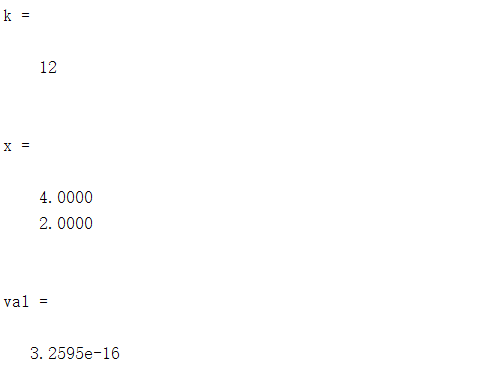
\includegraphics[width=0.45\textwidth]{dc1.png}
		\caption{对称秩1法结果}
		\label{fig:fig1}
	\end{figure}
	\subsection{BFGS算法}
	\indent 输入: fun,gfun分别是目标函数及其梯度,$x_0$是初始点,varargin是输入的可变参数变量,简单调用BFGS是可以忽略\\
	\indent 输出:k是迭代次数,x,val分别是近似最优点和最优值
	\begin{lstlisting}
	function [k,x,val] = bfgs(fun,gfun,x0,varargin)
	N=1000;
	epsilon=1.e-5;
	beta=0.55; sigma=0.4;
	n=length(x0); Bk=eye(n);
	k=0;
	while(k<N)
		gk=feval(gfun,x0,varargin{:});
		if(norm(gk)<epsilon), break; end 
		dk=-Bk\gk;
		m=0; mk=0;
		while(m<20)
			newf=feval(fun,x0+beta^m*dk,varargin{:});
			oldf=feval(fun,x0,varargin{:});
			if(newf<=oldf+sigma*beta^m*gk'*dk)
				mk=m; break;
			end
			m=m+1;
		end
		x=x0+beta^mk*dk;
		sk=x-x0;
		yk=feval(gfun,x,varargin{:})-gk;
		if(yk'*sk>0)
		Bk=Bk-(Bk*sk*sk'*Bk)/(sk'*Bk*sk)+(yk*yk')/(yk'*sk);
		end
		k=k+1;
		x0=x;
	end
	val=feval(fun,x0,varargin{:});
	end
	\end{lstlisting}
	\indent 在对称秩1算法问题的基础上,命令窗口输入
	\begin{lstlisting}
	>> x0=[1.0;1.0];
	>> [k,x,val]=bfgs('fun1','gfun1',x0)
	\end{lstlisting}
		\begin{figure}[ht]
		\centering
		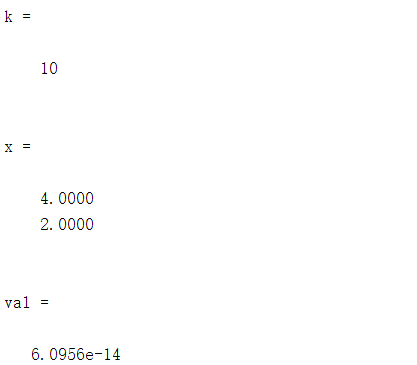
\includegraphics[width=0.38\textwidth]{bfgs.png}
		\caption{BFGS算法结果}
		\label{fig:fig1}
	\end{figure}
	\subsection{DFP算法}
	\indent 输入: fun,gfun分别是目标函数及其梯度,$x_0$是初始点,
	epsilon是容许误差,N是最大迭代次数\\
	\indent 输出:k是迭代次数,x,val分别是近似最优点和最优值
	\begin{lstlisting}
	function [k,x,val] = dfp(fun,gfun,x0,epsilon,N)
	if nargin<5, N=1000; end
	if nargin<4, epsilon=1.e-5; end
	beta=0.55; sigma=0.4;
	n=length(x0); Hk=eye(n); k=0;
	while(k<N)
		gk=feval(gfun,x0);
		if(norm(gk)<epsilon), break; end
		dk=-Hk*gk;
		m=0; mk=0;
		while(m<20)
			if(feval(fun,x0+beta^m*dk)<=feval(fun,x0)...
			+sigma*beta^m*gk'*dk)
			mk=m; break;
		end
		m=m+1;
		end
		x=x0+beta^mk*dk;
		sk=x-x0; yk=feval(gfun,x)-gk;
		if(sk'*yk>0)
		Hk=Hk-(Hk*yk*yk'*Hk)/(yk'*Hk*yk)+(sk*sk')/(sk'*yk);
		end
		k=k+1; x0=x;
	end
	val=feval(fun,x0);
	end
	\end{lstlisting}
	\indent 在对称秩1算法问题的基础上,命令窗口输入
	\begin{lstlisting}
	>> x0=[1.0;1.0];epsilon=1e-5;N=20;
	>> [k,x,val] = dfp('fun1','gfun1',x0,epsilon,N)
	\end{lstlisting}
	\begin{figure}[ht]
	\centering
	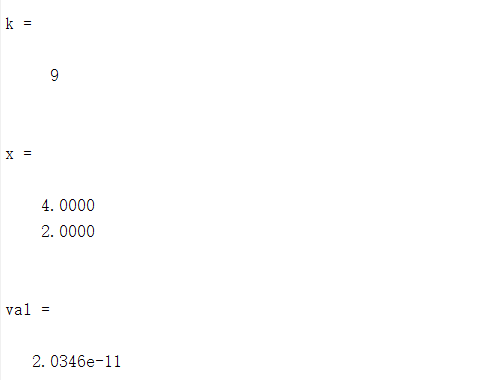
\includegraphics[width=0.45\textwidth]{dfp.png}
	\caption{DFP算法结果}
	\label{fig:fig1}
	\end{figure}
	\subsection{Broyden族算法}
	\indent 输入: fun,gfun分别是目标函数及其梯度,$x_0$是初始点,
epsilon是容许误差,N是最大迭代次数\\
	\indent 输出:k是迭代次数,x,val分别是近似最优点和最优值
	\begin{lstlisting}
	function [k,x,val] = broyden(fun,gfun,x0,epsilon,N)
	if nargin<5, N=1000; end
	if nargin<4, epsilon=1.e-5; end
	beta=0.55; sigma=0.4; phi=0.5;
	n=length(x0); Hk=eye(n); k=0;
	while(k<N)
		gk=feval(gfun,x0);
		if(norm(gk)<epsilon), break; end
		·dk=-Hk*gk;
		m=0; mk=0;
		while(m<20)
			if(feval(fun,x0+beta^m*dk)<=feval(fun,x0)...
			+sigma*beta^m*gk'*dk)
				mk=m; break;
			end
			m=m+1;
		end
		x=x0+beta^mk*dk; sk=x-x0;
		yk=feval(gfun,x)-gk; Hy=Hk*yk;
		sy=sk'*yk; yHy=yk'*Hk*yk;
		if(sy<0.2*yHy)
			theta=0.8*yHy/(yHy-sy);
			sk=theta*sk+(1-theta)*Hy;
			sy=0.2*yHy;
		end
		vk=sqrt(yHy)*(sk/sy - Hy/yHy);
		Hk=Hk-(Hy*Hy')/yHy+(sk*sk')/sy+phi*vk*vk';
		x0=x; k=k+1;
	end
	val=feval(fun,x0);
	end
	\end{lstlisting}
	\indent 在对称秩1算法问题的基础上,命令窗口输入
	\begin{lstlisting}
	>> x0=[1.0;1.0];epsilon=1e-5;N=20;
	>> [k,x,val]=broyden('fun1','gfun1',x0,epsilon,N)
	\end{lstlisting}
	\begin{figure}[ht]
	\centering
	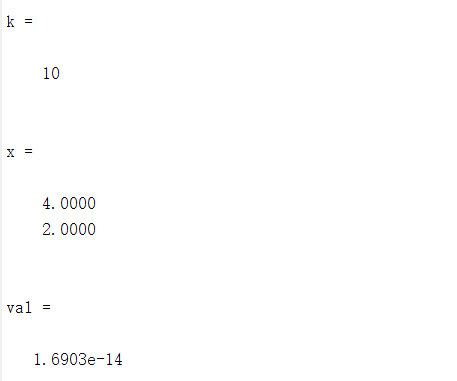
\includegraphics[width=0.45\textwidth]{broyden.png}
	\caption{Broyden算法结果}
	\label{fig:fig1}
	\end{figure}
	\section{信赖域算法}
	\subsection{光滑牛顿法求解信赖域子问题}
	\indent 输入:$f_k$是$x_k$处的目标函数值,$g_k$是$x_k$处的梯度,$B_k$是第k次近似Hesse阵,$\Delta_k$是当前信赖域半径\\
	\indent 输出:d,val分别是子问题的最优点和最优值,lam是乘子值,i是迭代次数
	\begin{lstlisting}
	function [d,val,lam,i] = trustq(fk,gk,Bk,deltak)
	n=length(gk); beta=0.6; sigma=0.2;
	mu0=0.05; lam0=0.05; gamma=0.05;
	d0=ones(n,1); z0=[mu0,lam0,d0']';
	zbar=[mu0,zeros(1,n+1)]';
	i=0;
	z=z0; mu=mu0; lam=lam0; d=d0;
	while (i<=150)
		H=dah(mu,lam,d,gk,Bk,deltak);
		if(norm(H)<=1.e-8)
			break;
		end
		J=JacobiH(mu,lam,d,Bk,deltak);
		b=psi(mu,lam,d,gk,Bk,deltak,gamma)*zbar-H;
		dz=J\b;
		dmu=dz(1); dlam=dz(2); dd=dz(3:n+2);
		m=0; mi=0;
		while (m<20)
			t1=beta^m;
			Hnew=dah(mu+t1*dmu,lam+t1*dlam,d+t1*dd,...
					gk,Bk,deltak);
			if(norm(Hnew)<=(1-sigma*(1-gamma*mu0)*beta^m)...
				*norm(H))
				mi=m; break;
			end
			m=m+1;
		end
		alpha=beta^mi;
		mu=mu+alpha*dmu;
		lam=lam+alpha*dlam;
		d=d+alpha*dd;
		i=i+1;
	end
	val=fk+gk'*d+0.5*d'*Bk*d;
	end
	%%
	function p=phi(mu,a,b)
	p=a+b-sqrt((a-b)^2+4*mu^2);
	end
	%%
	function H=dah(mu,lam,d,gk,Bk,deltak)
	n=length(d);
	H=zeros(n+2,1);
	H(1)=mu;
	H(2)=phi(mu,lam,deltak^2-norm(d)^2);
	H(3:n+2)=(Bk+lam*eye(n))*d+gk;
	end
	%%
	function J=JacobiH(mu,lam,d,Bk,deltak)
	n=length(d);
	J=zeros(n+2,n+2);
	t2=sqrt((lam+norm(d)^2-deltak^2)^2+4*mu^2);
	pmu=-4*mu/t2;
	thetak=(lam+norm(d)^2-deltak^2)/t2;
	J=[1, 0, zeros(1,n);
	pmu, 1-thetak, -2*(1+thetak)*d';
	zeros(n,1), d, Bk+lam*eye(n)];
	end
	%%
	function si=psi(mu,lam,d,gk,Bk,deltak,gamma)
	H=dah(mu,lam,d,gk,Bk,deltak);
	si=gamma*norm(H)*min(1,norm(H));
	end
	\end{lstlisting}
	\indent 结果可视化:\\
   	\indent 求解信赖域子问题最优解$\underset{||d||_2\le \Delta_k}{min} f(x)=-5+g_k^\mathrm{T}d+\frac{1}{2}d^\mathrm{T}B_kd$\\
	\indent 式中:
	$g_k=\begin{pmatrix}
		400\\
		-200
	\end{pmatrix}$,
	$B_k=\begin{pmatrix}
	1202 & -400\\
	-400 & 200
	\end{pmatrix}$,$\Delta_k=5$\\
	\indent 命令窗口输入:
	\begin{lstlisting}
	>> fk=-5;gk=[400 -200]';
	>> Bk=[1202 -400; -400 200];
	>> deltak=5;
	>> [d,val,lam,i] = trustq(fk,gk,Bk,deltak)
	\end{lstlisting}
	\begin{figure}[ht]
	\centering
	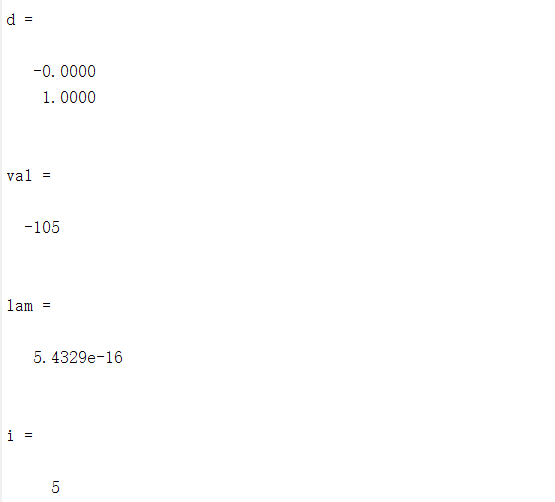
\includegraphics[width=0.45\textwidth]{trustq.png}
	\caption{光滑牛顿算法求解信赖域子问题结果}
	\label{fig:fig1}
	\end{figure}
	\subsection{牛顿型信赖域方法}
	\indent $x_0$是初始点,epsilon是容许误差\\
	\indent 输出:k是迭代次数,x,val分别是近似极小点和近似极小值
	\begin{lstlisting}
	function [k,x,val] = trustm(x0,epsilon)
	n=length(x0); eta1=0.1; eta2=0.75;
	tau1=0.5; tau2=2.0;
	delta=1; dtabar=2.0;
	x=x0; Bk=Hess(x);k=0;
	while(k<50)
		fk=fun(x);
		gk=gfun(x);
		if(norm(gk)<epsilon)
			break;
		end
		[d,val,lam,i]=trustq(fk,gk,Bk,delta);
		deltaq=fk-val;
		deltaf=fun(x)-fun(x+d);
		rk=deltaf/deltaq;
		if(rk<=eta1)
			delta=tau1*delta;
		else if (rk>=eta2 & norm(d)==delta)
				delta=min(tau2*delta,dtabar);
			else
				delta=delta;
			end
		end
		if(rk>eta1)
			x=x+d;
			Bk=Hess(x);
		end
		k=k+1;
	end
	val=fun(x);
	end
	\end{lstlisting}
	\indent 求解无约束优化问题 $\underset{x\in R^2}{min} f(x)=100(x_1^2-x_2)^2+(x_1-1)^2$\\
	\indent 编写fun.m,gfun.m,Hess.m
	\begin{lstlisting}
	%%
	function f=fun1(x)
	f=100*(x(1)^2-x(2))^2+(x(1)-1)^2;
	end
	%%
	function gf=gfun1(x)
	gf=[400*x(1)*(x(1)^2-x(2))+2*(x(1)-1); -200*(x(1)^2-x(2))];
	end
	%%
	function He=Hess1(x)
	He=[1200*x(1)^2-400*x(2)+2, -400*x(1);
	-400*x(1), 200 ];
	end
	\end{lstlisting}
	\indent 结果可视化:命令窗口输入
	\begin{lstlisting}
	>> x0=[0.0;0.0];epsilon=1e-6;
	>> [k,x,val] = trustm(x0,epsilon)
	\end{lstlisting}
	\begin{figure}[ht]
		\centering
		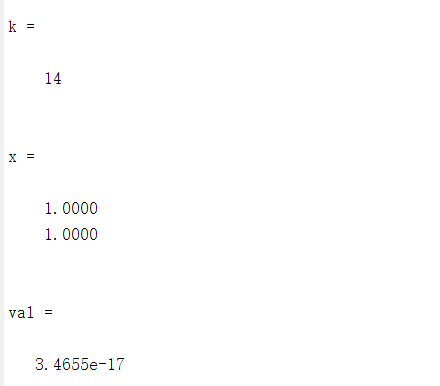
\includegraphics[width=0.45\textwidth]{trustm.png}
		\caption{牛顿型信赖域算法结果}
		\label{fig:fig1}
	\end{figure}
	\section{最小二乘法}
	\subsection{线性最小二乘问题}
	\subsubsection{法方程Cholesky分解法}
	\begin{lstlisting}
	function [x,res]=nels(A,b)
	B=A'*A; f=A'*b;
	L=chol(B,'lower');
	y=L\f; x=L'\y;
	res=norm(b-A*x);
	end
	\end{lstlisting}
	\indent 求解超定方程组 $Ax=b$,其中\\
	\indent $$A=\begin{pmatrix}
		2 & 3 & 4 & 5\\
		4 & 3 & 2 & 1\\
		4 & 5 & 6 & 7\\
		9 & 5 & 7 & 2\\
		4 & 2 &5 & 3
	\end{pmatrix},
	x=\begin{pmatrix}
		x1\\
		x2\\
		x3\\
		x4
	\end{pmatrix},
	b=\begin{pmatrix}
		20\\
		22\\
		35\\
		42\\
		50
	\end{pmatrix}$$
	\indent 命令窗口输入:
	\begin{lstlisting}
	>> A=[2 3 4 5; 4 3 2 1; 4 5 6 7; 9 5 7 2; 4 2 5 3];
	>> b=[20 22 35 42 50]';
	>> [x,res]=nels(A,b)
	\end{lstlisting}
	\begin{figure}[ht]
		\centering
		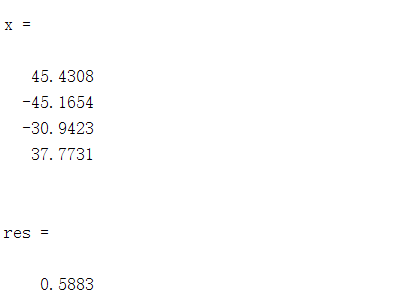
\includegraphics[width=0.4\textwidth]{nels.png}
		\caption{Cholesky分解结果}
		\label{fig:fig1}
	\end{figure}
	\subsubsection{QR分解法}
	\begin{lstlisting}
	function [x,res]=qrls(A,b)
	[Q,R]=qr(A); f=Q'*b;
	x=R\f; res=norm(b-A*x);
	end
	\end{lstlisting}
	\indent 求解Cholesky中的超定方程组\\
	\indent 命令窗口输入:
	\begin{lstlisting}
	>> A=[2 3 4 5; 4 3 2 1; 4 5 6 7; 9 5 7 2; 4 2 5 3];
	>> b=[20 22 35 42 50]';
	>> [x,res]=qrls(A,b)
	\end{lstlisting}
	\begin{figure}[ht]
		\centering
		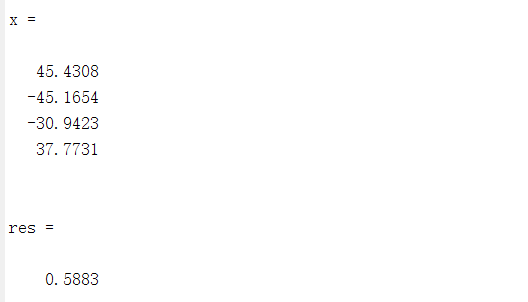
\includegraphics[width=0.45\textwidth]{qrls.png}
		\caption{QR分解结果}
		\label{fig:fig1}
	\end{figure}
	\subsubsection{SVD求解亏秩最小二乘}
	\begin{lstlisting}
	A=[1 2 3 4; 1 4 5 6; 1 5 6 7; 1 8 9 10; 1 11 12 13];
	b=[11 13 15 18 20]';
	[m,n]=size(A); x=zeros(n,1);
	[U,S,V]=svd(A);
	r=rank(S);
	for i=1:r
		x=x+(U(:,i)'*b/S(i,i))*V(:,i);
	end
	x
	res=norm(b-A*x)
	\end{lstlisting}
	\indent 求解超定方程组$Ax=b$,其中
$$A=\begin{pmatrix}
	1 & 2 & 3 & 4\\
	1 & 4 & 5 & 6\\
	1 & 5 & 6 & 7\\
	1 & 8 & 9 & 0\\
	1 & 11 & 12& 13
\end{pmatrix},
x=\begin{pmatrix}
	x1\\
	x2\\
	x3\\
	x4
\end{pmatrix},
b=\begin{pmatrix}
	11\\
	13\\
	15\\
	18\\
	20
\end{pmatrix}$$
	\indent 运行可得结果
	\begin{figure}[ht]
	\centering
	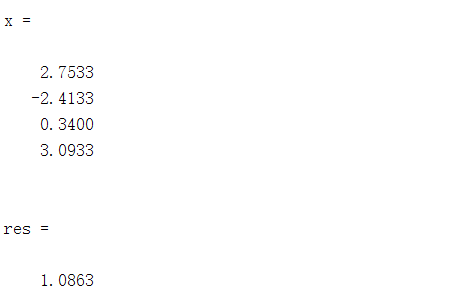
\includegraphics[width=0.45\textwidth]{svd.png}
	\caption{SVD分解结果}
	\label{fig:fig1}
	\end{figure}
	\subsection{非线性最小二乘问题}
	\subsubsection{L-M方法}
	求解非线性方程组$F(x)=0$,可适用于未知数个数与方程的个数不相等情形\\
	\indent 输入:$F_k,JF_k$分别是求F(xk)及F'(xk)的函数,$x_0$是初始点,epsilon是容许误差,N是最大迭代次数\\
	\indent 输出:k是迭代次数,x,val分别是近似解和$0.5*||F(xk)||^2$的值
	\begin{lstlisting}
	function [k,x,val] = lmm(Fk,JFk,x0,epsilon,N)
	if nargin<5, N=1000; end
	if nargin<4, epsilon=1.e-5; end
	beta=0.55; sigma=0.4;
	n=length(x0);
	muk=norm(feval(Fk,x0));
	k=0;
	while(k<N)
		fk=feval(Fk,x0);
		jfk=feval(JFk,x0);
		gk=jfk'*fk; dk=-(jfk'*jfk+muk*eye(n))\gk;
		if(norm(gk)<epsilon), break; end
		m=0; mk=0;
		while(m<20)
			fnew=0.5*norm(feval(Fk,x0+beta^m*dk))^2;
			fold=0.5*norm(feval(Fk,x0))^2;
			if(fnew<fold+sigma*beta^m*gk'*dk)
				mk=m; break;
			end
			m=m+1;
		end
		x0=x0+beta^mk*dk;
		muk=norm(feval(Fk,x0));
		k=k+1;
	end
	x=x0;
	val=0.5*muk^2;
	end
	\end{lstlisting}
	\indent 结果可视化:编写Fk.m和JFK.m
	\begin{lstlisting}
	%%
	function F=Fk(x)
	n=length(x); F=zeros(n,1);
	for i=1:n-1
		F(i)=x(i)*x(i+1)-1;
	end
	F(n)=x(1)*x(n)-1;
	%%
	function JF=JFk(x)
	n=length(x); JF=zeros(n,n);
	for i=1:n-1
		for j=1:n
			if j==i
				JF(i,j)=x(j+1);
			else if j==i+1
				JF(i,j)=x(j-1);
				else
					JF(i,j)=0;
				end
			end
		end
	end
	JF(n,1)=x(n); JF(n,n)=x(1);
	\end{lstlisting}
	\indent 命令窗口输入:
	\begin{lstlisting}
	>> x0=3*ones(100,1);epsilon=1e-6; N=20;
	>> [k,x,val] = lmm('Fk','JFk',x0,epsilon,N)
	\end{lstlisting}
\begin{figure}[ht]
	\centering
	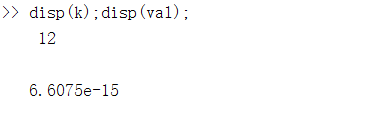
\includegraphics[width=0.45\textwidth]{lmm.png}
	\caption{LM方法结果}
	\label{fig:fig1}
\end{figure}
\end{document}